% =============================================================
\chapter{État de l'art}
\label{chap:state-of-the-art}
\selectlanguage{french}

\minitoc                  % mini-table du chapitre
\setlength{\parindent}{0pt}

% -----------------------------------------------------------------
% 2.1 Architecture des visuels Power BI
\section{Architecture des visuels Power BI}
\label{sec:archi-powerbi}

Power~BI est conçu autour d’une \textbf{architecture de visualisation ouverte
et extensible}.  
Chaque élément visuel (graphique, carte, jauge, etc.) est rendu côté client
à partir des données du modèle, via du code JavaScript/TypeScript exécuté
dans Power~BI Desktop ou dans le service web \parencite{MicrosoftOpenVis2015}.  
Depuis 2015, Microsoft propose non seulement une panoplie de visuels
« \emph{core} » (natifs), mais permet aussi l’importation de visuels
additionnels développés par la communauté ou des éditeurs tiers
\parencite{MicrosoftMarketplace2016}.  
Cette ouverture repose sur des standards web : \emph{« en s’appuyant sur des
standards ouverts d’Internet et des bibliothèques open-source comme D3.js »},
la création de visuels personnalisés a été grandement simplifiée
\parencite{MicrosoftD3Blog2017}.  
Microsoft publie d’ailleurs le code source de nombreux visuels natifs sur
GitHub, attestant de sa volonté d’encourager un écosystème ouvert
\parencite{GitHubPowerBISamples2024}.

%-----------------------------------------------------------
\subsection{Visual container et bac à sable}
\label{subsec:sandbox}
%-----------------------------------------------------------

Qu’il soit natif ou personnalisé, un visuel s’insère dans le \emph{canevas}
du rapport et interagit avec le modèle de données via des rôles prédéfinis.
Chaque visuel reçoit, du moteur Power BI, les données filtrées qui lui sont
attribuées (colonnes, mesures, hiérarchies), puis exécute son propre code de
rendu.  
Pour les visuels \emph{custom}, ce code est empaqueté dans un fichier
\verb|.pbiviz| contenant les scripts, les styles et le manifeste
\parencite{MicrosoftPbivizDocs2023}.  
Power BI exécute alors le visuel dans un \textbf{bac à sable sécurisé}
(\emph{sandbox}) : une \texttt{iframe} isolée du reste du rapport
\parencite{OkVizSandbox2022}.  
Le visuel n’accède ni aux autres visuels ni au modèle global ; il ne « voit »
que les champs que l’utilisateur lui a explicitement liés
\parencite{OkVizSandbox2022}.  
Cette mesure garantit qu’aucun code malveillant ne peut lire ou exfiltrer des
données sans autorisation \parencite{MediumSecurityPBI2023}.

%-----------------------------------------------------------
\subsection{Interactions et intégration}
\label{subsec:interactions}
%-----------------------------------------------------------

Malgré cet isolement technique, les visuels s’intègrent pleinement dans
l’expérience interactive globale.  
Un visuel personnalisé correctement développé se comporte \emph{exactement
comme un visuel natif} : il réagit aux filtres, autorise le
\textit{cross-highlight} (mise en surbrillance croisée) et expose des options
de mise en forme dans le panneau \emph{Format}
\parencite{MicrosoftCustomVisGuide2024}.  
Lorsqu’un utilisateur clique, par exemple, sur une barre d’histogramme, le
moteur Power BI propage l’événement de sélection aux autres visuels.
Si le développeur a implémenté l’API \verb|ISelectionManager|, son visuel
peut émettre et recevoir ces événements, assurant ainsi une \textbf{intégration
uniforme} des visuels natifs et ajoutés \parencite{MicrosoftSelectionAPI2024}.  

La différence fondamentale reste donc interne : les visuels natifs font
partie du produit et peuvent exploiter des API internes non exposées,
tandis que les visuels personnalisés s’appuient uniquement sur
l’API publique du SDK, avec les restrictions de sécurité détaillées en
section~\ref{sec:sdk}.

% 2.2 Visuels natifs : analyse fonctionnelle
\section{Visuels natifs : capacités et limites}
\label{sec:natifs-powerbi}

Avant d'envisager la création de visuels personnalisés via Python, R ou le SDK TypeScript, il convient de dresser un panorama complet des visuels dits \emph{natifs} disponibles dans Power BI. Ceux-ci sont préinstallés et activement maintenus par Microsoft, couvrant la majorité des besoins courants en analyse et restitution de données. Cette section propose non seulement une typologie complète, mais aussi une lecture critique de leur rôle et de leurs limites dans un contexte professionnel.

\subsection{Typologie fonctionnelle des visuels standards}

\subsubsection{Graphiques de comparaison}
Barres et colonnes (groupées, empilées, 100~\%) permettent de visualiser des agrégations comparées entre catégories. Elles acceptent le tri dynamique et le forage hiérarchique (drill-down) jusqu'au niveau de granularité le plus fin. Leur usage est optimal pour des tableaux de bord orientés suivi de performance, mais reste limité par l'absence de sous-totaux intermédiaires et la rigidité des axes (un seul axe secondaire).

\subsubsection{Graphiques de tendance}
Les courbes et aires (simples, empilées, 100~\%) modélisent des séries temporelles ou continues. Idéales pour l'analyse temporelle de KPI, les courbes supportent l'affichage d'un axe secondaire, et les aires mettent en valeur les volumes cumulés. Leur capacité de drill-down et de filtrage croisé les rend adaptées à des rapports interactifs.

\subsubsection{Graphiques combinés}
Les visuels de type ``combo'' (barres + lignes) permettent de superposer par exemple un chiffre d'affaires mensuel et une marge en pourcentage. Ils sont recommandés lorsque deux échelles de mesure doivent coexister dans un même visuel, sans multiplier les graphiques.

\subsubsection{Graphique de ruban}
Spécifique à la représentation du \emph{rang}, le graphique de ruban est adapté à l'analyse de parts de marché dynamiques. Il est utile pour suivre les changements de position relative de catégories dans le temps (produits, régions, marques).

\subsubsection{Graphiques de processus}
\emph{Cascade} (waterfall) permet de visualiser des variations successives contribuant à un total, tandis que \emph{entonnoir} (funnel) illustre les déperditions d'un processus (par exemple ventes ou parcours client). Le waterfall accepte les sous-totaux intermédiaires, contrairement à l'entonnoir.

\subsubsection{Nuages de points et bulles}
Le scatter plot est utile pour explorer les corrélations entre deux variables quantitatives. L'ajout d'une dimension via la taille de la bulle permet des lectures croisées. Ces visuels sont pertinents pour des analyses exploratoires mais se heurtent à une limite de volume : au-delà de 30\,000 points, l’agrégation est imposée.

\subsubsection{Graphiques circulaires}
Secteurs (pie) et anneaux (donut) représentent les parts d'un total. Bien que fréquemment utilisés, ils sont à réserver à un nombre réduit de segments (idéalement $<6$) sous peine de perte de lisibilité. Leur usage reste plus esthétique que fonctionnel.

\subsubsection{Treemaps et arborescences}
Les treemaps permettent d'encapsuler plusieurs niveaux hiérarchiques dans une surface limitée. Leur lecture est efficace pour les structures catégorielles denses (portefeuilles produits, répartitions géographiques). Un clic fore dans la hiérarchie, avec mise en forme conditionnelle possible.

\subsubsection{Cartographie}
\begin{itemize}
  \item \textbf{Carte Bing} : affiche des bulles proportionnelles sur fond routier ; recommandée pour des localisations simples.
  \item \textbf{Carte remplie (choroplèthe)} : colore les régions selon une valeur agrégée ; utile pour les données administratives.
  \item \textbf{Azure Maps} : propose une cartographie vectorielle moderne avec gestion de clusters et carte thermique.
  \item \textbf{ArcGIS for Power BI} : permet des fonctions spatiales avancées (zones isochrones, couches socio-démographiques), avec certaines restrictions sans compte Esri.
\end{itemize}

\subsubsection{Cartes de KPI et jauges}
\begin{itemize}
  \item \textbf{Carte (single)} : affiche une métrique unique, très lisible sur petits écrans.
  \item \textbf{Carte multi-lignes} : combine plusieurs KPIs dans un seul composant.
  \item \textbf{KPI} : présente une valeur, une cible et une tendance ; bien adapté au suivi d’objectifs.
  \item \textbf{Jauge} : visualisation qualitative d’une performance vs objectif ; limitée à un usage mono-métrique.
\end{itemize}

\subsubsection{Tableaux et matrices}
Les tableaux affichent les données ligne à ligne ; les matrices pivotent les dimensions et permettent les totaux intermédiaires. Pour des rapports très formatés, Power BI propose \emph{le rapport paginé} (RDL), utile dans un contexte administratif.

\subsubsection{Filtres interactifs}
\textbf{Segments (slicers)} : composants filtrants par catégorie, plage ou date. Le segment bouton améliore l’ergonomie sur mobile et permet une navigation par clic visuel.

\subsubsection{Visuels d'intelligence artificielle}
\begin{itemize}
  \item \textbf{Influenceurs clés} : détecte les dimensions explicatives d’une mesure cible.
  \item \textbf{Arborescence de décomposition} : propose des détails successifs de manière semi-automatisée.
  \item \textbf{Q\&A} : traduit une requête en langage naturel en visuel dynamique.
  \item \textbf{Narratif intelligent} : génère du texte automatisé en fonction des filtres actifs.
\end{itemize}

\subsubsection{Intégrations actionnables}
\begin{itemize}
  \item \textbf{Power Apps visual} : intègre une app canvas interactive pour actions en base (formulaires, validation).
  \item \textbf{Power Automate visual} : ajoute un bouton qui lance un processus automatisé (email, mise à jour CRM).
\end{itemize}

\subsection*{Analyse critique}

\paragraph{Points forts}
\begin{itemize}
  \item Performance optimale : chargement rapide, compatibilité multi-plateforme.
  \item Maintenance assurée : mise à jour automatique et fiabilité.
  \item Accessibilité native : compatibilité avec les lecteurs d'écran et thèmes d'entreprise.
  \item Intégration simple : aucun développement requis.
\end{itemize}

\paragraph{Limitations clés}
\begin{itemize}
  \item Faible personnalisation : interface de configuration figée.
  \item Interactivité limitée à ce que prévoit Microsoft ; pas de logique conditionnelle.
  \item Structure tabulaire obligatoire : peu adapté aux modèles de graphes, répétitions ou réseaux.
  \item Pas d’accès au DOM, au code ou aux \texttt{event listeners}.
\end{itemize}

\subsection*{Conclusion intermédiaire}
Les visuels natifs forment un socle de démarrage fiable, rapide et adapté à 80~\% des besoins analytiques en entreprise. Cependant, leur manque de souplesse les rend insuffisants pour des besoins de personnalisation graphique avancée, d’interactivité dynamique ou d’intégration à des architectures complexes. C’est précisément dans ces cas que les visuels personnalisés (Python, R, SDK) prennent toute leur valeur.


% 2.3 Visuels scriptés Python / R
%-----------------------------------------------------------
\section{Visuels Python / R : usages, atouts, limites}
\label{sec:python-r-visuals}
%-----------------------------------------------------------

Outre les visuels préfabriqués, Power BI autorise l’exécution de scripts Python ou R pour produire des visuels sur mesure.  
L’utilisateur insère un composant « Python visual » ou « R visual » dans le canevas, saisit le code dans un éditeur intégré, puis Power BI exécute ce script en tâche de fond : les données liées sont transmises sous forme de DataFrame et le résultat retourné est une image statique (PNG) affichée dans le rapport.

Cette fonctionnalité exploite l’écosystème analytique complet de chaque langage : Matplotlib, Seaborn ou Plotly côté Python ; ggplot2 ou plotly R côté R.  
Un data-scientist peut, en quelques lignes, tracer dans Power BI un nuage de points avec régression \textsc{Loess} (R) ou un diagramme de réseau (Python) — visuels impossibles à obtenir via les graphes natifs, notamment quand l’Arbre de décomposition limite la profondeur d’analyse et n’accepte qu’une seconde mesure \parencite{MicrosoftDecompositionTree2024}.

\begin{figure}[h]
  \centering
  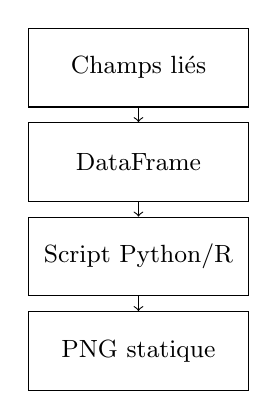
\begin{tikzpicture}[node distance=1.2cm, every node/.style={font=\small}]
    \node (bind) [draw, rectangle, minimum width=2.8cm, minimum height=1cm] {Champs liés};
    \node (df)   [below of=bind, draw, rectangle, minimum width=2.8cm, minimum height=1cm] {DataFrame};
    \node (code) [below of=df,   draw, rectangle, minimum width=2.8cm, minimum height=1cm] {Script Python/R};
    \node (png)  [below of=code, draw, rectangle, minimum width=2.8cm, minimum height=1cm] {PNG statique};
    \draw[->] (bind) -- (df);
    \draw[->] (df)   -- (code);
    \draw[->] (code) -- (png);
  \end{tikzpicture}
  \caption{Pipeline d’exécution d’un visuel Python / R dans Power BI}
  \label{fig:python-r-pipeline}
\end{figure}

\subsection{Atouts analytiques}

L’accès direct aux bibliothèques open-source autorise statistiques avancées, clustering, apprentissage automatique, carte de chaleurs ou dendrogrammes ; le script peut pré-traiter les données ou entraîner un modèle avant de générer le graphique.  
À chaque rafraîchissement, l’exécution se relance automatiquement : l’utilisateur bénéficie ainsi de calculs que DAX ou Power Query ne permettent pas aisément, par exemple l’analyse de texte ou les séries temporelles non linéaires.

\subsection{Limites techniques et fonctionnelles}

Le résultat demeure une image statique — « les visualisations Python dans Power BI sont des bitmaps 72 DPI, sans interactivité directe » \parencite{MicrosoftPythonRVisualsDocs2024}.  
Impossible donc d’initier un filtrage croisé depuis le graphique ; seul un filtre externe relance le script.  
Power BI transmet au script au plus 150 000 lignes, alloue 250 Mio de mémoire et impose un temps plafond de cinq minutes en local, soixante secondes dans le service ; la sortie PNG des visuels R est limitée à 2 Mio \parencite{MicrosoftRPackagesService2025}.  
Le runtime cloud, actuellement R 4.3.3 et Python 3.11, restreint le package compressé à 30 Mio, et l’affichage de ces visuels exige une licence Pro ou un workspace Premium : un utilisateur Free ne les verra pas.

\subsection{Enjeux de sécurité et de maintenance}

Power BI signale explicitement qu’un visuel Python ou R contient du code exécutable arbitraire \parencite{MicrosoftPythonRVisualsDocs2024}.  
Dans un environnement professionnel, cela impose une gouvernance rigoureuse : le script, encapsulé dans le fichier binaire .pbix, échappe au suivi Git ; il doit donc être extrait dans un dépôt versionné afin de permettre la traçabilité et la revue par les pairs. De plus, le runtime cloud (Python 3.11, R 4.3.3) ainsi que ses bibliothèques sont mis à jour automatiquement chaque mois ; un fichier requirements.txt (ou renv.lock pour R) et des tests de régression sont indispensables pour vérifier la compatibilité après chaque release. Enfin, puisque ces scripts disposent d’un accès direct au système de fichiers et au réseau, il convient de restreindre leurs privilèges (comptes de service à droits minimaux, liste blanche de packages) afin de prévenir toute exfiltration de données ou exécution de code malveillant.

\subsection{Bilan et positionnement stratégique}

Les visuels Python et R offrent un recours efficace pour des analyses spécialisées ponctuelles, mais la nature statique du rendu, les contraintes de performance et les exigences de licence limitent leur usage à grande échelle.  
Une comparaison détaillée entre visuels natifs, Python/R et SDK figurera dans le tableau synthétique de la section \ref{sec:synthese}; on y montrera que, pour un besoin récurrent et interactif, le développement d’un visuel SDK représente l’alternative la plus pérenne pour ECRINS SA.


% 2.4 SDK Power BI : structure, sécurité, pipeline

\section{SDK Custom Visuals : principes, sécurité et pipeline}
\label{sec:sdk-custom-visuals}

Le Software Development Kit (SDK) pour visuels personnalisés de Power BI permet de créer des composants graphiques entièrement sur mesure en TypeScript, répondant précisément à des besoins analytiques, interactifs ou visuels très spécifiques. Cette section détaille les principes de développement, les aspects sécuritaires à respecter, ainsi que les bonnes pratiques pour gérer un pipeline d’intégration et de déploiement continu (CI/CD).

\subsection{Principes généraux du développement via SDK}

Le développement d’un visuel personnalisé avec le SDK Power BI implique les étapes suivantes :
\begin{enumerate}
  \item Initialisation du projet via l’outil \texttt{pbiviz} (ligne de commande).
  \item Définition des capacités du visuel via le fichier \texttt{capabilities.json}.
  \item Implémentation en TypeScript dans \texttt{src/visual.ts} en suivant l'interface \texttt{IVisual}.
  \item Gestion du rendu graphique à l’aide de bibliothèques comme D3.js, React ou autres frameworks JavaScript.
  \item Compilation et packaging du visuel en fichier \texttt{.pbiviz} prêt à être déployé.
\end{enumerate}

Le SDK impose une structure modulaire claire, facilitant la maintenance et l’évolution du composant au fil des besoins et des versions du rapport.

\subsection{Sécurité et isolation des visuels custom}

Power BI exécute chaque visuel personnalisé dans une sandbox HTML sécurisée (iframe). Ce mécanisme garantit l’isolation complète du code personnalisé par rapport au reste du rapport, protégeant ainsi :
\begin{itemize}
  \item Contre les conflits de bibliothèques JavaScript (versions incompatibles).
  \item Contre les failles potentielles (accès non autorisé au DOM principal).
  \item En limitant strictement les échanges à travers une API contrôlée (sélections, filtres croisés, thèmes).
\end{itemize}

Depuis la version 4.6 du SDK, il est obligatoire de déclarer explicitement les privilèges et autorisations nécessaires (fichiers externes, accès réseau) dans le fichier \texttt{capabilities.json}. Ces contraintes assurent une transparence complète en matière de sécurité et facilitent l'audit des visuels déployés dans un environnement de production.

\subsection{Pipeline CI/CD pour les visuels custom}

Pour industrialiser efficacement le développement et le déploiement des visuels personnalisés, la mise en place d’un pipeline d’intégration et de déploiement continu (CI/CD) est recommandée. Ce pipeline typique inclut les étapes suivantes :
\begin{itemize}
  \item \textbf{Intégration continue (CI)} :
  \begin{itemize}
    \item Validation automatique des changements via des tests unitaires et fonctionnels.
    \item Compilation du projet TypeScript avec vérification des erreurs et des standards de codage.
    \item Génération automatique du package \texttt{.pbiviz} pour chaque commit.
  \end{itemize}
  \item \textbf{Déploiement continu (CD)} :
  \begin{itemize}
    \item Déploiement automatique du visuel sur des environnements de test puis de production.
    \item Automatisation des étapes de vérification de sécurité et d'intégration.
    \item Gestion simplifiée des versions via le contrôle de source (Git, Azure DevOps, GitHub Actions).
  \end{itemize}
\end{itemize}

Ce processus garantit une haute qualité logicielle, une traçabilité complète des modifications, et une réduction drastique des risques liés à des mises en production manuelles ou ponctuelles.

\subsection{Bonnes pratiques et conseils de mise en œuvre}

Pour réussir le développement de visuels personnalisés avec le SDK Power BI, il est essentiel de suivre quelques recommandations clés :
\begin{itemize}
  \item \textbf{Structure claire du code} : Séparer distinctement la logique métier (traitement de la dataView) de la logique d’affichage (D3.js, Canvas).
  \item \textbf{Tests rigoureux} : Couvrir au maximum les méthodes critiques avec des tests unitaires et d’intégration (Jest, Mocha).\
  \item \textbf{Documentation exhaustive} : Documenter clairement le fonctionnement du visuel, les options disponibles et les limites éventuelles pour faciliter l’intégration par les équipes de développement ou les utilisateurs finaux.
  \item \textbf{Optimisation performance} : Privilégier un rendu différentiel (update incrémental), utiliser des méthodes efficaces pour la gestion des grands jeux de données.
\end{itemize}

\subsection*{Conclusion intermédiaire}

Le SDK Custom Visuals de Power BI offre une solution optimale pour répondre à des besoins spécifiques dépassant les capacités natives ou les limites des visuels Python et R. Grâce à son cadre structurant, ses exigences de sécurité élevées, et son potentiel d’automatisation via CI/CD, il représente la meilleure option pour un usage professionnel à grande échelle. Ce choix technologique s’impose particulièrement lorsque la performance, l’interactivité dynamique, et la personnalisation graphique poussée sont des critères essentiels du projet BI.


% 2.5 Choix technologiques (TypeScript, D3, React ?)
\section{Choix technologiques : TypeScript, D3, (option React)}
\label{sec:technos}

Créer un visuel Power BI custom revient essentiellement à développer une application web monopage embarquée. À ce titre, le choix des technologies de développement est déterminant pour réussir à la fois l’implémentation technique et la maintenabilité du code. À l’heure actuelle (2023--2025), un consensus s’est formé autour du trio technologique suivant pour les visuels Power BI : TypeScript comme langage de développement, D3.js comme bibliothèque de visualisation de bas niveau, et éventuellement React (ou un autre framework UI) pour structurer l’interface si nécessaire. Ces choix ne sont pas exclusifs — en principe, le SDK permet l’usage de n’importe quel framework JavaScript du moment qu’il peut s’intégrer dans le bundle en module ES6 \cite{reddit-es6} — mais ils reflètent les recommandations et pratiques courantes dans la communauté.

\subsection{TypeScript comme langage par défaut}

Le SDK Power BI est conçu pour TypeScript, un sur-ensemble typé de JavaScript. Lorsqu’on initialise un projet de visuel, les fichiers générés (ex. \texttt{visual.ts}, \texttt{settings.ts}) sont en TypeScript \cite{ms-sdk-typescript}. L’adoption de TypeScript présente plusieurs avantages :
\begin{itemize}
  \item typage statique permettant d’attraper des erreurs à la compilation ;
  \item meilleure productivité grâce à l’autocomplétion et à la documentation dans les IDE ;
  \item interopérabilité totale avec JavaScript.
\end{itemize}
Microsoft fournit les définitions d’interfaces du Power BI Visuals API en TypeScript, ce qui facilite le développement. Un développeur purement JavaScript pourrait théoriquement coder un visuel, mais il perdrait les bénéfices du typage \cite{reddit-typescript-api}.

\subsection{D3.js pour le rendu visuel}

D3.js (Data-Driven Documents) est une bibliothèque JavaScript utilisée pour créer des visualisations en SVG/Canvas. Microsoft a misé sur D3 dès l’origine des custom visuals : « en s’appuyant sur des librairies open-source comme D3.js, nous avons rendu la création de nouveaux visuels incroyablement simple » \cite{powerbi-d3}. La majorité des visuels personnalisés utilisent D3, qui permet de relier les données au DOM. D3 est agnostique, léger, et déjà intégré dans l’environnement Power BI : « D3 est attaché au contexte global de la sandbox, ce qui le rend immédiatement disponible » \cite{fabric-d3-sandbox}.

\subsection{React (optionnel) pour la structure UI}

L’utilisation de React est possible mais non systématique. De nombreux visuels simples n’en ont pas besoin. Cependant, React devient pertinent pour :
\begin{itemize}
  \item les visuels complexes avec état interne (menus, boutons, événements) ;
  \item la réutilisation de composants existants ;
  \item les équipes déjà familières avec React.
\end{itemize}
Microsoft propose un tutoriel officiel sur l’usage de React dans les visuels custom \cite{ms-react-circlecard}. Toutefois, React n’est pas parfaitement intégré dans le sandbox Power BI, et nécessite des ajustements spécifiques. Des développeurs ont signalé des problèmes liés au \texttt{window} sandboxé, et Microsoft a confirmé que le contexte global est isolé pour des raisons de sécurité \cite{fabric-react-sandbox}.

\subsection{Autres technologies et alternatives}

D’autres bibliothèques peuvent être utilisées : Chart.js, Vega-Lite, Plotly.js, voire Three.js pour des besoins spécifiques (cartographie, 3D, etc.). Des solutions comme Deneb ou Charticulator permettent aussi de créer des visuels sans coder, tout en s’appuyant en interne sur D3.

\subsection{Choix pour le projet}

Dans le cadre du projet pour ECRINS SA, le choix de TypeScript et D3.js est privilégié pour leur robustesse, leur compatibilité et leur capacité à répondre à des besoins métier précis. React ne sera envisagé que si des interactions avancées sont nécessaires. Ce trio technologique permettra de produire des visuels performants, intégrables et conformes aux bonnes pratiques.



% =============================================================
